\documentclass[screen]{beamer}
\usepackage[T1]{fontenc}
\usepackage[utf8]{inputenc}
\usepackage{listings}
\usetheme{ntnuenglish}
\usepackage[english]{babel}
\usepackage[pdftex]{graphicx}
\usepackage{sidecap}

\title{TDT4240: Component-based Game Engine}

\author[finnrobi, sibtehai, tornes]{Sibte-Haider Syed\\
  Dag Øyvind Tornes\\
  Robin Kåveland Hansen}

\date{}

\lstset{basicstyle=\tiny,
  numbers=left,
  stepnumber=1,
  showstringspaces=false
  }

\begin{document}
\ntnutitlepage

\begin{frame}
  \frametitle{Agenda}
  \begin{itemize}
    \item Context
    \item Architecture
    \item Evaluation of architecture
    \item Cool things that architecture supports
  \end{itemize}
\end{frame}

\begin{frame}
  \frametitle{Chosen project}
  \begin{itemize}
    \item Chose XNA as our COTS
    \item Wanted to make game inspired by:
      \begin{itemize}
        \item Tower Defense
        \item Geometry Wars 
        \item RPGs (DotA + similar)
        \item 2D arcade spaceshooter hero defense RPG!
      \end{itemize}
    \item Quality Attribute focus was Modifiability
    \item Secondary Attribute was Usability
    \item Extensibility by data-driven architecture
  \end{itemize}
\end{frame}

\begin{frame}
  \frametitle{Commit activity by day and hour}
  \begin{figure}
    \includegraphics[scale=0.35]{activity}
    \caption{Size of circle = number of commits in timeslot}
  \end{figure}
\end{frame}

\begin{frame}
  \frametitle{Project structure}
  3 separate Visual Studio projects\\
  \begin{itemize}
    \item Code for the game itself
    \item Models (Describes data formats for XNA)
    \item Data (XML data files, sprites)
  \end{itemize}
  Used Git for Version Control of all projects\\
  Visual Studio Plugin: Git Extensions
\end{frame}

\begin{frame}
  \frametitle{Architectural solution}
  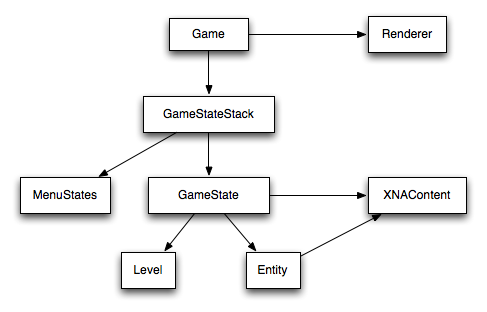
\includegraphics[scale=0.5]{classes}
\end{frame}

\begin{frame}
  \frametitle{About entities...}
  \begin{columns}
    \begin{column}{0.6\linewidth}
      Behaviour defined by properties\\
      Loaded from XML data files\\
      Some properties are controllers\\
      Most act as models\\
      Composed of small classes\\
      Most only have 2-3 methods\\
    \end{column}
    \begin{column}{0.4\linewidth}
      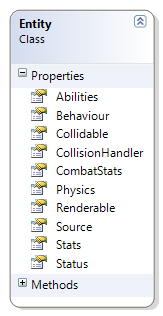
\includegraphics[scale=0.7]{../reports/graphics/entity}
    \end{column}
  \end{columns}
\end{frame}

\begin{frame}
  \frametitle{Example of an EntityModel}
  \lstinputlisting[language=xml]{example.xml}
\end{frame}

\begin{frame}
  \frametitle{Cool things this lets us do}
  \emph{Or the things we wish we had time for}
  \begin{itemize}
    \item Compose new kinds of enemies that use existing abilities
    \item Architecture lets us embed a scripting language / console
      \begin{itemize}
        \item Lua is possible to embed in C\#
        \item Wanted to, but ran out of time
      \end{itemize}
    \item Could script bosses / enemies at runtime...
    \item Levels and enemies are data, easy to create new
    \item Add many cool abilities
    \item Script some bosses
    \item Allow for savegame by serializing entities...
    \item Create some actual art
    \item Add sounds
  \end{itemize}
\end{frame}

\end{document}
